\documentclass[12pt,utf8,notheorems,compress,t]{beamer}
\usepackage{etex}

\usepackage{pgfpages}
\setbeameroption{show notes on second screen}
\setbeamertemplate{note page}[plain]
\newcommand{\jnote}[2]{\only<#1>{\note{\setlength\parskip{\medskipamount}\justifying\footnotesize#2\par}}}

% Workaround for the issue described at
% https://tex.stackexchange.com/questions/164406/beamer-using-href-in-notes.
\newcommand{\fixedhref}[2]{\makebox[0pt][l]{\hspace*{\paperwidth}\href{#1}{#2}}\href{#1}{#2}}

\usepackage[english]{babel}

\usepackage{mathtools}
\usepackage{booktabs}
\usepackage{stmaryrd}
\usepackage{array}
\usepackage{ragged2e}
\usepackage{multicol}
\usepackage{tabto}
\usepackage{xstring}
\usepackage{ifthen}
\usepackage{soul}\setul{0.3ex}{}
\usepackage[all]{xy}
\xyoption{rotate}
\usepackage{tikz}
\usetikzlibrary{calc,shapes,shapes.callouts,shapes.arrows,patterns,fit,backgrounds,decorations.pathmorphing}
\hypersetup{colorlinks=true}

\usepackage{pifont}
\newcommand{\cmark}{\ding{51}}
\newcommand{\xmark}{\ding{55}}
\DeclareSymbolFont{extraup}{U}{zavm}{m}{n}
\DeclareMathSymbol{\varheart}{\mathalpha}{extraup}{86}

\graphicspath{{images/}}

\usepackage[protrusion=true,expansion=true]{microtype}

\setlength\parskip{\medskipamount}
\setlength\parindent{0pt}

\title{New reduction techniques in commutative algebra driven by logical methods}
\author{Ingo Blechschmidt}
\date{October 24th, 2018}

\useinnertheme[shadow=true]{rounded}
\setbeamerfont{block title}{size={}}

\useinnertheme{rectangles}

\usecolortheme{orchid}
\usecolortheme{seahorse}
\definecolor{mypurple}{RGB}{150,0,255}
\setbeamercolor{structure}{fg=mypurple}
\definecolor{myred}{RGB}{150,0,0}
\setbeamercolor*{title}{bg=myred,fg=white}
\setbeamercolor*{titlelike}{bg=myred,fg=white}
\setbeamercolor{frame}{bg=black}

\usefonttheme{serif}
\usepackage[T1]{fontenc}
\usepackage{libertine}

\newcommand{\A}{\mathcal{A}}
\newcommand{\B}{\mathcal{B}}
\newcommand{\M}{\mathcal{M}}
\renewcommand{\AA}{\mathbb{A}}
\newcommand{\E}{\mathcal{E}}
\newcommand{\F}{\mathcal{F}}
\renewcommand{\G}{\mathcal{G}}
\newcommand{\J}{\mathcal{J}}
\newcommand{\GG}{\mathbb{G}}
\renewcommand{\O}{\mathcal{O}}
\newcommand{\K}{\mathcal{K}}
\newcommand{\NN}{\mathbb{N}}
\newcommand{\QQ}{\mathbb{Q}}
\newcommand{\RR}{\mathbb{R}}
\newcommand{\TT}{\mathbb{T}}
\newcommand{\PP}{\mathbb{P}}
\newcommand{\ZZ}{\mathbb{Z}}
\newcommand{\CC}{\mathbb{C}}
\renewcommand{\P}{\mathcal{P}}
\newcommand{\aaa}{\mathfrak{a}}
\newcommand{\ppp}{\mathfrak{p}}
\newcommand{\fff}{\mathfrak{f}}
\newcommand{\defeq}{\vcentcolon=}
\newcommand{\defeqv}{\vcentcolon\equiv}
\newcommand{\Sh}{\mathrm{Sh}}
\newcommand{\GL}{\mathrm{GL}}
\newcommand{\Zar}{\mathrm{Zar}}
\newcommand{\op}{\mathrm{op}}
\newcommand{\Set}{\mathrm{Set}}
\newcommand{\Eff}{\mathrm{Ef{}f}}
\newcommand{\Sch}{\mathrm{Sch}}
\newcommand{\Aff}{\mathrm{Aff}}
\newcommand{\Ring}{\mathrm{Ring}}
\newcommand{\LocRing}{\mathrm{LocRing}}
\newcommand{\LRS}{\mathrm{LRS}}
\newcommand{\Hom}{\mathrm{Hom}}
\newcommand{\Spec}{\mathrm{Spec}}
\newcommand{\lra}{\longrightarrow}
\newcommand{\RelSpec}{\operatorname{Spec}}
\renewcommand{\_}{\mathpunct{.}}
\newcommand{\?}{\,{:}\,}
\newcommand{\speak}[1]{\ulcorner\text{\textnormal{#1}}\urcorner}
\newcommand{\ull}[1]{\underline{#1}}
\newcommand{\affl}{\ensuremath{{\ull{\AA}^1}}}
\newcommand{\Ll}{\vcentcolon\!\Longleftrightarrow}
\newcommand{\inv}{inv.\@}
\newcommand{\seq}{\vdash_{\!\!\!\vec x}}

\setbeamertemplate{blocks}[rounded][shadow=false]

\newenvironment{indentblock}{%
  \list{}{\leftmargin\leftmargin}%
  \item\relax
}{%
  \endlist
}

% Adapted from https://latex.org/forum/viewtopic.php?t=2251 (Stefan Kottwitz)
\newenvironment<>{hilblock}{
  \begin{center}
    \begin{minipage}{9.05cm}
      \setlength{\textwidth}{9.05cm}
      \begin{actionenv}#1
        \def\insertblocktitle{}
        \par
        \usebeamertemplate{block begin}}{
        \par
        \usebeamertemplate{block end}
      \end{actionenv}
    \end{minipage}
  \end{center}}

\newcommand{\bignumber}[1]{
  \renewcommand{\insertenumlabel}{#1}\scalebox{1.5}{\usebeamertemplate{enumerate item}}
}
\newcommand{\bigheart}{
\includegraphics{heart}}

\newenvironment{changemargin}[2]{%
  \begin{list}{}{%
    \setlength{\topsep}{0pt}%
    \setlength{\leftmargin}{#1}%
    \setlength{\rightmargin}{#2}%
    \setlength{\listparindent}{\parindent}%
    \setlength{\itemindent}{\parindent}%
    \setlength{\parsep}{\parskip}%
  }%
  \item[]}{\end{list}}

\tikzset{
  invisible/.style={opacity=0,text opacity=0},
  visible on/.style={alt={#1{}{invisible}}},
  alt/.code args={<#1>#2#3}{%
    \alt<#1>{\pgfkeysalso{#2}}{\pgfkeysalso{#3}}}
}

\newcommand{\pointthis}[3]{%
  \tikz[remember picture,baseline]{
    \node[anchor=base,inner sep=0,outer sep=0] (#2) {#2};
    \node[visible on=#1,overlay,rectangle callout,rounded corners,callout relative pointer={(0.3cm,0.5cm)},fill=blue!20] at ($(#2.north)+(-0.1cm,-1.1cm)$) {#3};
  }%
}

% Adapted from https://latex.org/forum/viewtopic.php?t=2251 (Stefan Kottwitz)
\newenvironment<>{varblock}[2]{\begin{varblockextra}{#1}{#2}{}}{\end{varblockextra}}
\newenvironment<>{varblockextra}[3]{
  \begin{center}
    \begin{minipage}{#1}
      \begin{actionenv}#4
        {\centering \hil{#2}\par}
	\def\insertblocktitle{}%\centering #2}
        \def\varblockextraend{#3}
	\usebeamertemplate{block begin}}{
        \par
        \usebeamertemplate{block end}
        \varblockextraend
      \end{actionenv}
    \end{minipage}
  \end{center}}

\setbeamertemplate{frametitle}{%
  \vskip1.2em%
  \leavevmode%
  \begin{beamercolorbox}[dp=1ex,center]{}%
      \usebeamercolor[fg]{item}{\textbf{{\Large \insertframetitle}}}
  \end{beamercolorbox}%
}

\setbeamertemplate{navigation symbols}{}

\newcounter{framenumberpreappendix}
\newcommand{\backupstart}{
  \setcounter{framenumberpreappendix}{\value{framenumber}}
}
\newcommand{\backupend}{
  \addtocounter{framenumberpreappendix}{-\value{framenumber}}
  \addtocounter{framenumber}{\value{framenumberpreappendix}} 
}

\newcommand{\mynav}[3]{%
  \begin{beamercolorbox}[wd=\paperwidth,ht=2.25ex]{}%
    \begin{columns}
      \begin{column}{0.333\textwidth}
        \raggedright
        \textcolor{#1}{\qquad\qquad Summary}
        \par
      \end{column}
      \begin{column}{0.333\textwidth}
        \centering
        \textcolor{#2}{The forcing model}
        \par
      \end{column}
      \begin{column}{0.333\textwidth}
        \raggedleft
        \textcolor{#3}{Revisiting the test cases \qquad\qquad}
        \par
      \end{column}
    \end{columns}
  \end{beamercolorbox}%
}

\newcommand{\insertframeextra}{}
\setbeamertemplate{footline}{%
  \begin{beamercolorbox}[wd=\paperwidth,ht=2.25ex,dp=1ex,right,rightskip=1mm,leftskip=1mm]{}%
    % \inserttitle
    \hfill
    \insertframenumber\insertframeextra\,/\,\inserttotalframenumber
  \end{beamercolorbox}%
  \vskip0pt%
}


\newcommand{\hil}[1]{{\usebeamercolor[fg]{item}{\textbf{#1}}}}
\newcommand{\bad}[1]{\textcolor{red!90}{\textnormal{#1}}}

\begin{document}

\addtocounter{framenumber}{-1}

\setbeamertemplate{headline}{\mynav{gray}{gray}{gray}}

{\usebackgroundtemplate{\begin{minipage}{\paperwidth}\vspace*{4.95cm}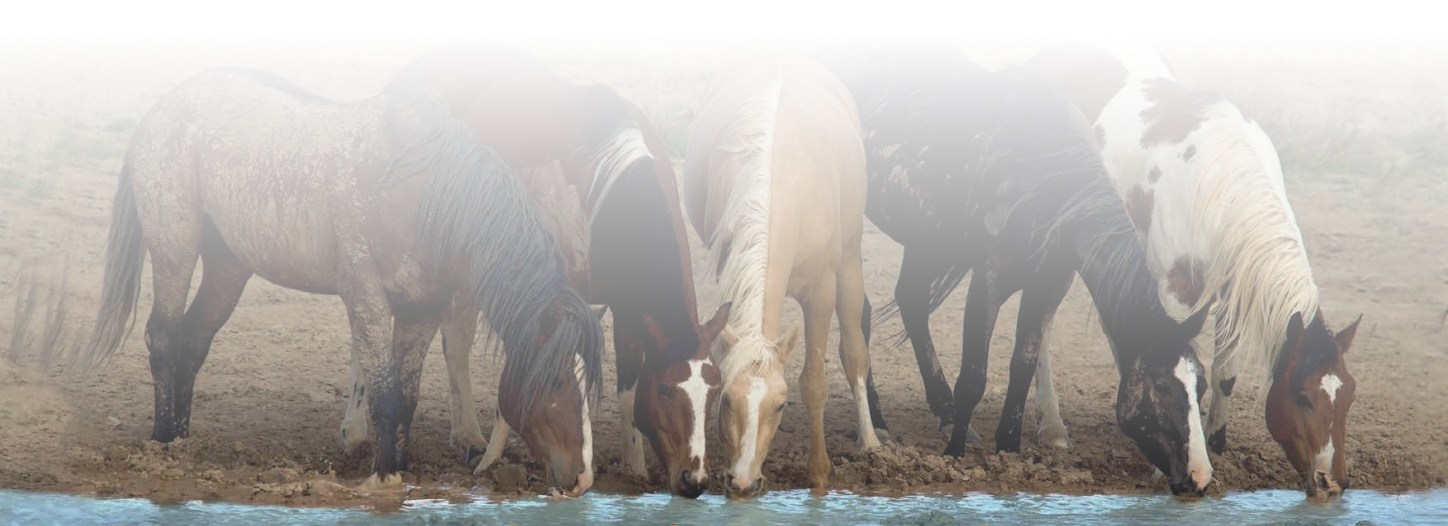
\includegraphics[width=\paperwidth]{topos-horses}\end{minipage}}
\begin{frame}[c]
  \centering

  \bigskip
  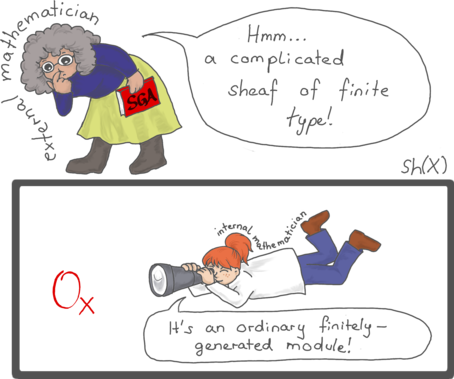
\includegraphics[width=0.4\textwidth]{external-internal-small}
  \bigskip

  \hil{New reduction techniques in commutative algebra driven by logical methods}

  \scriptsize
  \textit{-- an invitation --}
  \bigskip

  Ingo Blechschmidt \\
  Università di Verona
  \bigskip

  Logic Seminar Padova \\
  December 5st, 2018
  \par
\end{frame}}


\section{Summary}
\setbeamertemplate{headline}{\mynav{black}{gray}{gray}}

\begin{frame}{Summary}
  \vspace*{-1em}

  \visible<4>{
    \begin{changemargin}{-2.0em}{-0.5em}
      \begin{itemize}
        \item \ \\[-1.2em]\mbox{For any reduced ring~$A$, there is a ring~$A^\sim$ in a certain topos with}
        \[ \models \bigl(\forall x\?A^\sim\_ \neg(\exists y\?A^\sim\_ xy = 1) \Rightarrow x = 0\bigr). \]

        \item This semantics is sound with respect to intuitionistic logic.

        \item \ \\[-1.2em]\mbox{It has uses in classical and constructive commutative
        algebra.}
      \end{itemize}
    \end{changemargin}
  }

  \vspace*{-1.5em}

  \begin{columns}[t]
    \begin{column}[t]{0.52\textwidth}
      \centering

      \begin{varblock}{\textwidth}{A baby example}
        \justifying
        Let~$M$ be an injective matrix with more columns than rows over a
        reduced ring~$A$.
        Then~$1 = 0$ in~$A$.
      \end{varblock}
      \vspace*{-0.5em}

      \only<1>{
        \scalebox{0.8}{$\begin{pmatrix}
          \cdot & \cdot & \cdot & \cdot & \cdot \\
          \cdot & \cdot & \cdot & \cdot & \cdot \\
          \cdot & \cdot & \cdot & \cdot & \cdot
        \end{pmatrix}$}
      }

      \visible<2->{
        \justifying
        \textbf{Proof.} \bad{Assume not.} Then there is a \bad{minimal
        prime ideal} $\ppp \subseteq A$. The matrix is injective over the \bad{field}~$A_\ppp = A[(A
        \setminus \ppp)^{-1}]$; contradiction to basic linear algebra.
      }
    \end{column}

    \begin{column}[t]{0.46\textwidth}
      \centering

      \begin{varblock}{\textwidth}{Generic freeness\phantom{p}}
        \justifying
        Generically, any finitely generated module over a reduced ring
        is free.\phantom{g}
      \end{varblock}
      \vspace*{-0.5em}

      \only<1-2>{{
        \scriptsize\raggedright
        (A ring is reduced iff $x^n=0$ implies $x=0$.)
        \par
      }}

      \only<1-2>{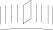
\includegraphics[width=0.73\textwidth]{generic-freeness}}

      \visible<3->{
        \justifying
        \textbf{Proof.} See \href{https://stacks.math.columbia.edu/tag/051Q}{[Stacks Project]}.
      }
    \end{column}
  \end{columns}

  \jnote{1}{The two displayed statements are trivial for fields. It is
  therefore natural to try to reduce the general situation to the field
  situation.}

  \jnote{2}{The displayed proof, which could have been taken from any
  standard textbook on commutative algebra, succeeds in this reduction
  by employing proof by contradition and minimal prime ideals. However, this way
  of reducing comes at a cost: It requires the Boolean Prime Ideal Theorem
  (for ensuring the existence of a prime ideal and for ensuring that stalks at
  minimal prime ideals are fields) and even the full axiom of choice (for
  ensuring the existence of a minimal prime ideal).

  We should hope that such a simple statement admits a more informative,
  explicit, computational proof: There should be an explicit method for
  transforming the given conditional equations expressing injectivity into the
  equation~$1 = 0$. And indeed there is: Beautiful constructive proofs can
  be found in Richman's note on
  \fixedhref{https://www.ams.org/journals/proc/1988-103-04/S0002-9939-1988-0954974-5/S0002-9939-1988-0954974-5.pdf}{nontrivial
  uses of trivial rings} and in the
  \fixedhref{https://arxiv.org/abs/1605.04832}{recent textbook by Lombardi and
  Quitté} on constructive commutative algebra.

  The new reduction technique presented in this talk provides a way of
  performing the reduction in an entirely constructive manner, avoiding the
  axiom of choice. If so desired, resulting topos-theoretic proofs can be
  unwound to yield fully explicit, topos-free, direct proofs.}

  \jnote{3}{The baby example demonstrates that the reduction technique of this
  talk is of interest to constructive commutative algebra. What about classical
  commutative algebra? This is what the second example aims at.
  Grothendieck's generic freeness lemma is an important theorem in algebraic
  geometry, where it is usually stated in the following geometric form:

  \vspace*{-1.2em}
  \begin{indentblock}Let~$X$ be a reduced scheme. Let~$\B$ be
  an~$\O_X$-algebra of finite type. Let~$\M$ be a~$\B$-module of finite type.
  Then over a dense open,
  \begin{enumerate}
  \item[(a)] $\B$ and~$\M$ are locally free as sheaves of~$\O_X$-modules,
  \item[(b)] $\B$ is of finite presentation as a sheaf of~$\O_X$-algebras and
  \item[(c)] $\M$ is of finite presentation as a sheaf of~$\B$-modules.
  \end{enumerate}\end{indentblock}
  \vspace*{-1.2em}

  All previously known proofs proceed in a series of reduction steps,
  finally culminating in the case where~$A$ is a Noetherian integral domain.
  They are somewhat convoluted (spanning several pages) and require nontrivial
  prerequisites in commutative algebra.

  Using the new reduction technique, there is a short (one-paragraph) and
  conceptual proof of Grothendieck's generic freeness lemma. It is constructive
  as a bonus; and if desired, one can unwind the resulting proof to obtain a
  constructive proof which doesn't reference topos theory. The proof obtained
  in this way is still an improvement on the previously known proofs, requiring
  no advanced prerequisites in commutative algebra, and takes
  \fixedhref{https://arxiv.org/abs/1807.01231}{about a page}.}
\end{frame}


\section{The forcing model}
\setbeamertemplate{headline}{\mynav{gray}{black}{gray}}

\begin{frame}{Motivating the semantics}
  \centering
  \begin{varblockextra}{0.8\textwidth}{}{
    \hil{Examples:}\phantom{Non-}\,\!\ \ $k,\ k[[X]],\ \CC\{z\},\ \ZZ_{(p)}$ \\[0.2em]
    \hil{Non-examples:}\ \ $\ZZ,\ k[X],\ \ZZ/(pq)$
  }
    \justifying
    A ring is \hil{local} iff~$1 \neq 0$ and if~$x + y = 1$ implies that~$x$ is
    invertible or~$y$ is invertible.
  \end{varblockextra}

  \begin{varblockextra}{0.8\textwidth}{}{
    Let~$x + y = 1$ in a ring~$A$.
    Then:
    \begin{itemize}
      \item The element $x$ is invertible in~$A[x^{-1}]$.
      \item The element $y$ is invertible in~$A[y^{-1}]$.
    \end{itemize}
    (Recall~$A[f^{-1}] = \bigl\{ \frac{u}{f^n} \,|\, u \in A, n \in \NN \bigr\}$.)
  }
    \hil{Locally,} any ring is local.
  \end{varblockextra}

  \jnote{1}{In topos theory, we have lots of experience of ``changing
  universes'' in order to ``force'' some statements to be true. However,
  because the field condition we are aiming at is not a ``geometric sequent'', these
  techniques do not work here. Hence we try to take it more slowly and devise a
  semantics which forces the given ring only to be local.

  The key insight is that \emph{locally} (in the sense of topology/geometry),
  any ring is a local ring. That is, we may pretend that any given ring is
  local if we are prepared to pass to numerous localizations during the course
  of an argument. The semantics displayed on the next slide manages this
  localization-juggling for us.}
\end{frame}

\begin{frame}{The Kripke--Joyal semantics}
  \small\vspace*{-0.7em}
  \only<1>{Let~$A$ be a ring (commutative, with unit). We recursively define
  \[ f \models \varphi \quad \text{(``$\varphi$ holds away from the zeros of~$f$'')} \]
  for elements~$f \in A$ and statements~$\varphi$. Write
  ``$\models \varphi$'' to mean~$1 \models \varphi$.}
  \only<1>{\[ \renewcommand{\arraystretch}{1.25}\begin{array}{@{}l@{\quad}c@{\quad}l@{}}
    f \models \top &\text{is}& \text{true} \\
    f \models \bot &\text{iff}& \text{$f$ is nilpotent} \\
    f \models x = y &\text{iff}& x = y \in A[f^{-1}] \\
    f \models \varphi \wedge \psi &\text{iff}&
      \text{$f \models \varphi$ and $f \models \psi$} \\
    f \models \varphi \vee \psi &\text{iff}&
      \text{there exists a partition~$f^n = fg_1 + \cdots + fg_m$ with,} \\
    &&\quad\text{for each~$i$, $fg_i \models \varphi$ or $fg_i \models \psi$} \\
    f \models \varphi \Rightarrow \psi &\text{iff}&
      \text{for all~$g \in A$, $fg \models \varphi$ implies $fg \models \psi$} \\
    f \models \forall x\?A^\sim\_ \varphi &\text{iff}&
      \text{for all~$g \in A$ and all $x_0 \in A[(fg)^{-1}]$, $fg \models \varphi[x_0/x]$} \\
    f \models \exists x\?A^\sim\_ \varphi &\text{iff}&
      \text{there exists a partition~$f^n = fg_1 + \cdots + fg_m$ with,} \\
    &&\quad\text{for each~$i$, $fg_i \models \varphi[x_0/x]$ for some~$x_0 \in A[(fg_i)^{-1}]$}
  \end{array} \]}
  \only<2->{Write ``$\models \varphi$'' to mean~$1 \models \varphi$.}
  \only<2->{\[ \renewcommand{\arraystretch}{1.25}\begin{array}{@{}l@{\quad}c@{\quad}l@{}}
    f \models x = y &\text{iff}& x = y \in A[f^{-1}] \\
    f \models \varphi \wedge \psi &\text{iff}&
      \text{$f \models \varphi$ and $f \models \psi$} \\
    f \models \varphi \vee \psi &\text{iff}&
      \text{there exists a partition~$f^n = fg_1 + \cdots + fg_m$ with,} \\
    &&\quad\text{for each~$i$, $fg_i \models \varphi$ or $fg_i \models \psi$}
  \end{array} \]}

  \jnote{1}{The clause for~``$\vee$'' is made exactly in such a way as to
  ensure, if~$x + y = 1$, that~$1 \models ((\exists z\?A^\sim\_ xz = 1) \vee
  (\exists z\?A^\sim\_ yz = 1))$.
  
  The definition of the semantics is reminiscient of Kripke and Beth models.
  Indeed, it is a fragment of the Kripke--Joyal semantics of the \emph{internal
  language of a topos}, and this general semantics encompasses Kripke and Beth
  models as special cases.}

  \jnote{2}{The soundness lemma states: If~$f \models \varphi$, and
  if~$\varphi$ intuitionistically entails a further statement~$\psi$, then
  also~$f \models \psi$. In this way we can \emph{reason} with the forcing
  model, similarly as if~$A^\sim$ would actually exist as a ring instead of
  merely being a convenient syntactic fiction.

  If we want~$A^\sim$ to actually exist, not just as a figure of speech, then
  we have to broaden our notion of existence and accept ring objects in
  toposes. More on this on the next slide.

  Irrespective of whether~$A$ is a local ring, its mirror
  image~$A^\sim$ is always a local ring (that is, the axioms of what it means
  to be a local ring hold under the translation rules specified by the
  semantics). A basic application of this forcing model are local-to-global
  principles. For instance:
  \begin{itemize}\justifying
    \item The statement ``the kernel of a surjective matrix over a local ring
    is finite free'' admits a constructive proof. It therefore holds
    for~$A^\sim$. Its external meaning is that the kernel of a surjective
    matrix~$M$ over~$A$ is finite locally free (there exists a partition~$1 =
    f_1 + \cdots + f_n$ such that for each~$i$, the localized
    module~$(\operatorname{ker} M)[f_i^{-1}]$ is finite free).

    \item The ring~$A$ is a Prüfer domain if and only if~$A^\sim$ is a Bézout
    domain. Therefore any constructive theorem about Bézout domains entails a
    corresponding theorem about Prüfer domains. Bézout domains are quite rare,
    while Prüfer domains abound (for instance the ring of integers of any
    number field is a Prüfer domain, even constructively so).
  \end{itemize}}

  \pause

  \begin{columns}
    \begin{column}{0.50\textwidth}
      \begin{varblock}{\textwidth}{Monotonicity}{}
        If~$f \models \varphi$, then also~$fg \models \varphi$.
      \end{varblock}
    \end{column}

    \begin{column}{0.50\textwidth}
      \begin{varblock}{\textwidth}{Locality}{}
        \justifying
        If~$f^n = fg_1 + \cdots + fg_m$ and~$fg_i \models \varphi$ for all~$i$,
        then also~$f \models \varphi$.
      \end{varblock}
    \end{column}
  \end{columns}

  \begin{columns}
    \begin{column}{0.50\textwidth}
      \begin{varblock}{\textwidth}{Soundness\phantom{p}}{}
        If~$\varphi \vdash \psi$ and~$f \models \varphi$,
        then~$f \models \psi$.
      \end{varblock}
    \end{column}

    \begin{column}{0.50\textwidth}
      \begin{varblock}{\textwidth}{Forced properties}{}
        $\models \speak{$A^\sim$ is a local ring}$.
      \end{varblock}
    \end{column}
  \end{columns}
\end{frame}

\tikzstyle{topos} = [draw=mypurple, very thick, rectangle, rounded corners, inner sep=5pt, inner ysep=10pt]
\tikzstyle{title} = [fill=mypurple, text=white]

% Taken from Todd Lehman (CC-BY-SA) at https://tex.stackexchange.com/a/44920/32372

\newcommand{\setisprime}[1]{
  % Sets \isprime based on #1.
  \ifnum#1=1 \gdef\isprime{0} \else \gdef\isprime{1} \fi
  \foreach \sip in {2, 3,5,...,#1} {
    \pgfmathparse{\sip*\sip>#1? 1:0}
    \ifthenelse{\pgfmathresult=1}{
      % Early-out if \sip^2 > #1.
      \breakforeach
    }{
      % Otherwise test if \sip divides #1.
      \pgfmathparse{Mod(#1,\sip)==0? 1:0}
      \ifthenelse{\pgfmathresult=1}{
        \gdef\isprime{0}
        \breakforeach
      }{}
    }
  }
}

\newcommand{\setxy}[1]{
  % Sets \x and \y to loction of cell #1.
  \pgfmathtruncatemacro{\x}{Mod(#1-1,\cols)}
  \pgfmathtruncatemacro{\y}{(#1-1) / \cols}
  \pgfmathtruncatemacro{\y}{\cols - 1 - \y}
  \pgfmathparse{2.5*(\x+.5)}\let\x\pgfmathresult
  \pgfmathparse{2.5*(\y+.5)}\let\y\pgfmathresult
}

\newcommand{\numlabel}[2]{
  % Draws label #2 at cell #1.
  \setxy{\n}
  \node[fill=none, text=black] at (\x,\y) {#2};
}

\newcommand{\drawpolygon}[2]{
  % Draws polygon with #2 vertexes at cell #1.
  \setxy{#1}
  \ifthenelse{#2>1}{ % Polygon must have at least 2 sides.
    \ifthenelse{#2<30}{ % Draw polygon if it has a small number of sides.
      \filldraw (\x,\y) +(90:1)
      \foreach \drawi in {1,...,#2} {-- +(\drawi/#2*360+90:1)} -- cycle;
    }{ % Else approximate with circle.
      \filldraw (\x,\y) circle(1);
    }
  }{}
}

\newcommand{\setpolygoncolor}[1]{
  % Sets color based on #1.
  \gdef\polycolor{black}
  \ifnum#1=2\gdef\polycolor{black!50!white}\fi
  \ifnum#1=3\gdef\polycolor{yellow!95!red}\fi
  \ifnum#1=5\gdef\polycolor{yellow!0!red}\fi
  \ifnum#1=7\gdef\polycolor{blue!75!green}\fi
  \ifnum#1=11\gdef\polycolor{blue!70!red}\fi
  \ifnum#1=13\gdef\polycolor{blue!40!red}\fi
  \ifnum#1=17\gdef\polycolor{green!50!blue}\fi
  \ifnum#1=19\gdef\polycolor{green!80!black}\fi
  \ifnum#1=23\gdef\polycolor{green!50!red}\fi
  \ifnum#1=29\gdef\polycolor{yellow!50!black}\fi
  \ifnum#1=31\gdef\polycolor{orange!50!black}\fi
  \ifnum#1=37\gdef\polycolor{red!50!black}\fi
  \ifnum#1=41\gdef\polycolor{purple!50!black}\fi
  \ifnum#1=43\gdef\polycolor{blue!50!black}\fi
  \ifnum#1=47\gdef\polycolor{green!50!black}\fi
  \ifnum#1=53\gdef\polycolor{white!50!black}\fi
  \ifnum#1=59\gdef\polycolor{white!50!black}\fi
  \ifnum#1=61\gdef\polycolor{white!50!black}\fi
  \ifnum#1=67\gdef\polycolor{white!50!black}\fi
}

\newcommand{\sieve}[2]{
  \def\cols{#1}
  \def\rows{#2}
  \begin{tikzpicture}[scale=.5]
  \pgfmathtruncatemacro{\nmax}{\rows * \cols}

  \foreach \n in {1,...,\nmax} {
    \begin{scope}[fill=gray, fill opacity=.05,
                  draw=gray, draw opacity=.10,
                  line width=4]
      \drawpolygon{\n}{\n}
    \end{scope}
    \setisprime{\n}
    \ifthenelse{\isprime=1}{
      \numlabel{\n}{\bf\n}
    }{
      \def\startintensity{.33}
      \def\incrintensity{.10}
      \def\intensity{\startintensity}

      \def\m{\n}
      \pgfmathtruncatemacro{\i}{\m / 2}

      % Divide \m by \i until \m is extinguished.
      % Increment \i each time it does not divide into \m.
      \whiledo{\m>1}{
        \setisprime{\i}
        \pgfmathparse{Mod(\m,\i)==0? 1:0}
        \ifthenelse{\pgfmathresult=1\and\isprime=1}{
          \setpolygoncolor{\i}
          \begin{scope}[fill=\polycolor, fill opacity=\intensity,
                        draw=\polycolor!85!black, draw opacity=\intensity,
                        line width=\intensity*1.5]
            \drawpolygon{\n}{\i}
          \end{scope}
          \pgfmathtruncatemacro{\m}{\m / \i}
          \pgfmathparse{\intensity + \incrintensity}\let\intensity\pgfmathresult
        }{
          \pgfmathtruncatemacro{\i}{\i - 1}
          \def\intensity{\startintensity}
        }
      }
      \begin{scope}[text=black, text opacity=.5]
        \numlabel{\n}{\scriptsize\n}
      \end{scope}
    }
  }

  \end{tikzpicture}
}

%\renewcommand{\sieve}[2]{SIEVE}
%\renewcommand{\fakesieve}[2]{SIEVE}

\newcommand{\drawbox}[4]{
  \node[topos, #4] [fit = #3] (#1) {};
  \node[title] at (#1.north) {#2};
}

\newcommand{\muchstuff}{
  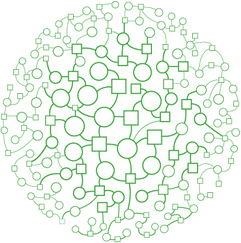
\includegraphics[height=3em]{filmat}
  \scalebox{0.5}{\sieve{14}{2}}
}

\newcommand{\muchstuffplaceholder}{
  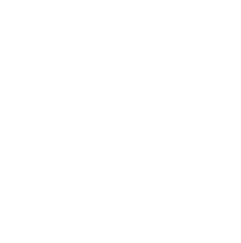
\includegraphics[height=3em]{filmat-placeholder}
  \scalebox{0.5}{\fakesieve{14}{2}}
}

\newcommand{\fewstuff}{
  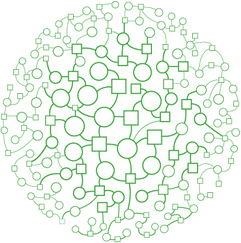
\includegraphics[height=3em]{filmat}
  \scalebox{0.5}{\sieve{7}{2}}
}

\begin{frame}[fragile]{A universal property}
  The displayed semantics is the first-order fragment of the \hil{higher-order
  internal language} of the \hil{little Zariski topos}.

  \begin{tikzpicture}
    \node[scale=0.4] (objs-set1) at (-4.0,-2.5) {
      \only<1->{\fewstuff}
    };
    \node[scale=0.4] (objs-eff1) at (4.0,-2.5) {
      \only<1->{\fewstuff}
    };
    \node[scale=0.4] (objs-sh1)  at (0,-2.5) {
      \only<1->{\fewstuff}
    };

    \node (prop-set1) [below of=objs-set1, align=left, inner ysep=0pt] {
      The usual laws \\
      of logic hold.
    };

    \node (prop-eff1) [below of=objs-eff1, align=left, inner ysep=0pt] {
      Every function \\
      is computable.
    };

    \node (prop-sh1) [below of=objs-sh1, align=left, inner sep=0pt] {
      The intermediate \\
      value theorem fails.
    };

    \begin{scope}
      \drawbox{set1}{$\mathrm{Set}$}{(objs-set1) (prop-set1)}{}
    \end{scope}
    \begin{scope}
      \drawbox{eff1}{Ef{}f}{(objs-eff1) (prop-eff1)}{tape}
    \end{scope}
    \begin{scope}
      \drawbox{sh1}{$\mathrm{Sh}\, X$}{(objs-sh1) (prop-sh1)}{draw=none}
      \def\R{8pt}
      \begin{pgfonlayer}{background}
      \draw[decoration={bumps,segment length=8pt}, decorate, very thick, draw=mypurple]
        ($(sh1.south west) + (\R, 0)$) arc(270:180:\R) --
        ($(sh1.north west) + (0, -\R)$) arc(180:90:\R) --
        ($(sh1.north east) + (-\R, 0)$) arc(90:0:\R) --
        ($(sh1.south east) + (0, \R)$) arc(0:-90:\R) --
        cycle;
      \end{pgfonlayer}
    \end{scope}
  \end{tikzpicture}

  \pause

  Is there a \hil{free local ring}~$A \to A'$ over~$A$?
  \begin{columns}[t]
    \begin{column}{0.4\textwidth}
      $\xymatrix{
        A \ar[rd] \ar[rrr]^\alpha &&& {\substack{\phantom{\text{local}}\\\text{\normalsize$R$}\\\text{local}}} \\
        & {\substack{\text{\normalsize$A'$}\\\text{local}}} \ar@{-->}_[@!35]{\text{local}}[rru]
      }$
    \end{column}

    \begin{column}{0.50\textwidth}
      \small\justifying
      For a fixed ring~$R$, the localization $A' \defeq A[S^{-1}]$ with $S \defeq
      \alpha^{-1}[R^\times]$ would do the job.
      \medskip

      Hence we need the \hil{generic filter}.
    \end{column}
  \end{columns}
\end{frame}

\begin{frame}{The little Zariski topos}
  \small

  Let~$A$ be a ring. Its \hil{little Zariski topos} is equivalently
  \vspace*{-0.5em}
  \begin{enumerate}
    \item the classifying locale of \hil{prime filters} of $A$, \\[-1.2em]
    \item the classifying topos of \hil{local localizations} of $A$, \\[-1.2em]
    \item the locale given by the frame of \hil{radical ideals} of $A$, \\[-1.2em]
    \item the topos of sheaves over the poset $A$ with $f \preceq g$ iff $f \in \sqrt{(g)}$ and with $(f_i \to f)_i$ deemed covering iff $f \in \sqrt{(f_i)_i}$ or \\[-1.2em]
    \item the topos of sheaves over $\Spec(A)$.
  \end{enumerate}
  Its associated topological space of points is the \hil{classical spectrum}
  \[ \{ \fff \subseteq A \,|\, \text{$\fff$ prime filter} \} + \text{Zariski topology}. \]
  It has \hil{enough points} if the Boolean Prime Ideal Theorem holds.

  \scriptsize
  Prime ideal:\, $0 \in \ppp$;\, $x \in \ppp \wedge y \in \ppp \Rightarrow x+y \in \ppp$;\, $1 \not\in \ppp$;\, $xy \in \ppp \Leftrightarrow x \in \ppp \vee y \in \ppp$

  Prime filter:\, $0 \not\in \fff$;\,\,
  $x+y \in \fff \Rightarrow x \in \fff \vee y \in \fff$;
  \hspace*{0.5pt}\,\,
  $1 \in \fff$;\,
  $xy \in \fff \Leftrightarrow x \in \fff \wedge y \in \fff$
\end{frame}

\begin{frame}{Investigating the forcing model}
% Let~$A$ be a reduced commutative ring ($x^n = 0 \Rightarrow x = 0$).
  \small

  The \hil{little Zariski topos} of a ring~$A$ is equivalently
  \vspace*{-0.5em}
  \begin{itemize}
    \item the topos of sheaves over~$\Spec(A)$, \\[-1.9em]
    \item the locale given by the frame of radical ideals of~$A$, \\[-1.9em]
%   \item the classifying topos of local localizations of~$A$ or
    \item the classifying locale of filters of~$A$
  \end{itemize}
  \vspace*{-0.5em}
  and contains a \hil{mirror image} of~$A$, the sheaf of rings $A^\sim$.

  \vspace*{-1.9em}

  \begin{columns}[t]
    \begin{column}{0.5\textwidth}
      \begin{varblock}{\textwidth}{}
        \justifying
        Assuming the Boolean Prime Ideal Theorem, a first-order
        formula ``$\forall \ldots \forall\_ (\cdots \Longrightarrow \cdots\!\,)$'',
        where the two subformulas may not contain~``$\Rightarrow$'' and~``$\forall$'',
        holds for~$A^\sim$ iff it holds for all stalks~$A_\ppp$.
      \end{varblock}

      \vspace*{-2em}

      \begin{varblock}{\textwidth}{}
        $A^\sim$ inherits any property of~$A$ which is
        \hil{localization-stable}.
      \end{varblock}
    \end{column}

    \begin{column}{0.5\textwidth}
      \vspace*{1.7em}

      If~$A$ is reduced ($x^n = 0 \Rightarrow x = 0$):

      \vspace*{-0.9em}
      \setbeamercolor{block body}{bg=red!30}
      \setbeamercolor{structure}{fg=purple}
      \begin{varblock}{\textwidth}{}
        $A^\sim$ is a \hil{field}.

        $A^\sim$ has \hil{$\boldsymbol{\neg\neg}$-stable equality}.

        \mbox{$A^\sim$ is \hil{anonymously Noetherian}.}\\[-1.2em]
      \end{varblock}
    \end{column}
  \end{columns}

  \visible<2->{\begin{tikzpicture}[overlay]
    \draw[fill=white, draw=white, opacity=0.85] (-1,0) rectangle (\paperwidth,8.0);
    \node[anchor=south west,inner sep=0] (image) at (0,1.0) {\vbox{
      \only<2>{
        \centering
        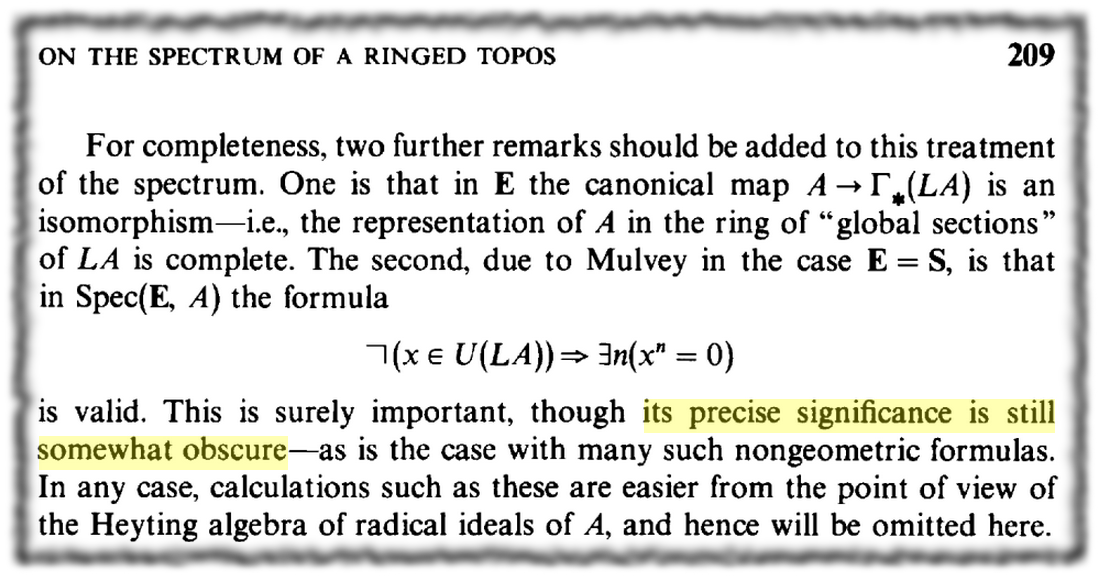
\includegraphics[width=0.9\textwidth]{tierney-on-the-spectrum-of-a-ringed-topos} \\
        \footnotesize
        Miles Tierney. On the spectrum of a ringed topos. 1976.
      }

      \only<3>{
	\begin{varblock}{\textwidth}{}
	  The external meaning of
	  \[
	    \models
	      \speak{$A^\sim[X_1,\ldots,X_n]$ is anonymously Noetherian}
	  \]
	  is:
	  \medskip

	  \begin{indentblock}
	  For any element~$f \in A$ and any (not necessarily quasicoherent) sheaf of
	  ideals~$\J \hookrightarrow A^\sim[X_1,\ldots,X_n]|_{D(f)}$: If
	  \begin{indentblock}
	  for any element~$g \in A$ the condition that
	  \begin{indentblock}
	  the sheaf~$\J$ is of finite type on~$D(g)$
	  \end{indentblock}
	  implies that~$g = 0$,
	  \end{indentblock}
	  then~$f = 0$.
	  \end{indentblock}
	\end{varblock}

	\vspace*{-2em}
      }
    }};
  \end{tikzpicture}}
\end{frame}
\renewcommand{\insertframeextra}{}


\section{Revisiting the test cases}
\setbeamertemplate{headline}{\mynav{gray}{gray}{black}}

\begin{frame}{Revisiting the test cases}
  \vspace*{-1em}
  Let~$A$ be a reduced commutative ring ($x^n = 0 \Rightarrow x = 0$). \\
  Let~$A^\sim$ be its mirror image in the little Zariski topos.

  \begin{columns}[t]
    \begin{column}[t]{0.48\textwidth}
      \centering

      \scalebox{0.5}{$\begin{pmatrix}
        \cdot & \cdot & \cdot & \cdot & \cdot \\
        \cdot & \cdot & \cdot & \cdot & \cdot \\
        \cdot & \cdot & \cdot & \cdot & \cdot
      \end{pmatrix}$}
      \vspace*{-0.5em}

      \begin{varblock}{\textwidth}{A baby example}
        \justifying
        Let~$M$ be an injective matrix over~$A$ with more columns than rows.
        Then~$1 = 0$ in~$A$.
      \end{varblock}

      \justifying
      \textbf{Proof.} $M$ is also injective as a matrix over~$A^\sim$.
      Since~$A^\sim$ is a field, this is a contradiction by basic linear
      algebra. Thus~$\models \bot$. This amounts to~$1 = 0$ in~$A$.
    \end{column}

    \begin{column}[t]{0.57\textwidth}
      \centering

      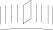
\includegraphics[height=1.9em]{generic-freeness}
      \vspace*{-0.5em}

      \begin{varblock}{\textwidth}{Generic freeness\phantom{p}}
        \justifying
        Let~$M$ be a finitely generated~$A$-module.
        If~$f = 0$ is the only element of~$A$ such that~$M[f^{-1}]$ is a
        free~$A[f^{-1}]$-module, then~$1 = 0$ in~$A$.
      \end{varblock}
      \vspace*{-0.1em}

      \justifying
      \textbf{Proof.} The claim amounts to \mbox{$\models
      \text{``$M^\sim$}$}$\text{
      is \hil{not not} free''}$. Since~$A^\sim$ is a field, this follows from
      basic linear algebra.
    \end{column}
  \end{columns}
\end{frame}


\backupstart
\setbeamertemplate{headline}{\mynav{gray}{gray}{gray}}

{\usebackgroundtemplate{\begin{minipage}{\paperwidth}\vspace*{4.95cm}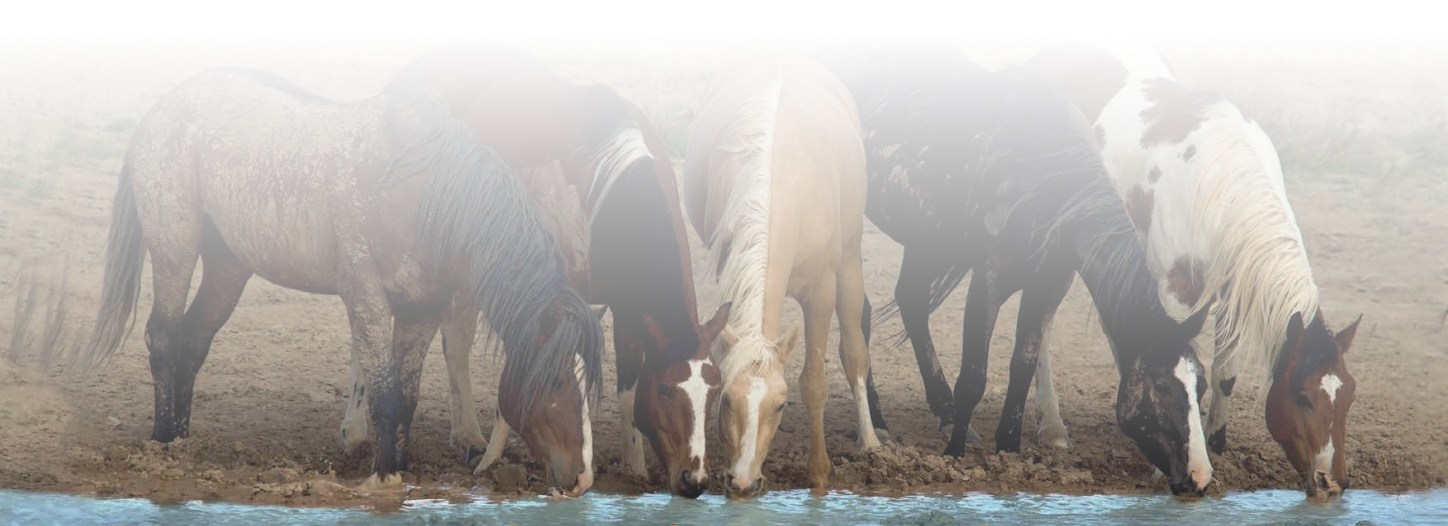
\includegraphics[width=\paperwidth]{topos-horses}\end{minipage}}
\begin{frame}
  \bigskip
  \centering
  
\includegraphics[height=3em]{heart}
  \par
  \raggedright

  The Zariski topos and related toposes have applications in:
  \begin{itemize}
    \item classical algebra and classical algebraic geometry
    \item constructive algebra and constructive algebraic geometry
    \item synthetic algebraic geometry (``schemes are just sets'')
  \end{itemize}

  Connections with:
  \begin{itemize}
    \item understanding quasicoherence
    \item the age-old mystery of nongeometric sequents
  \end{itemize}

\end{frame}}

\begin{frame}[plain,c]
  \centering%
  \hil{Further reading}
  \medskip

  \framebox{\href{https://pizzaseminar.speicherleck.de/skript2/zariski-topos-klein.pdf}{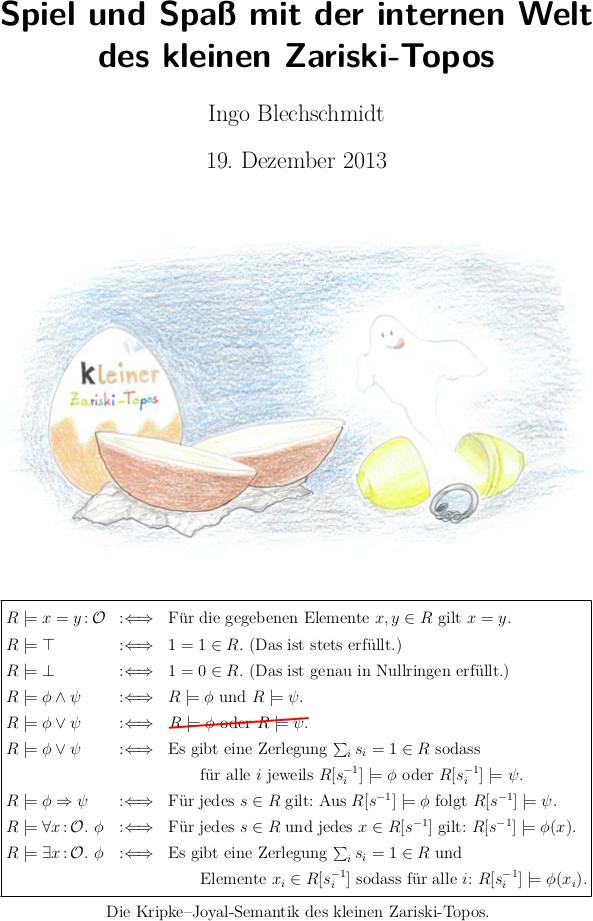
\includegraphics[height=0.8\textheight]{fun-with-the-zariski-topos}}}\qquad%
  \framebox{\href{https://rawgit.com/iblech/internal-methods/master/notes.pdf}{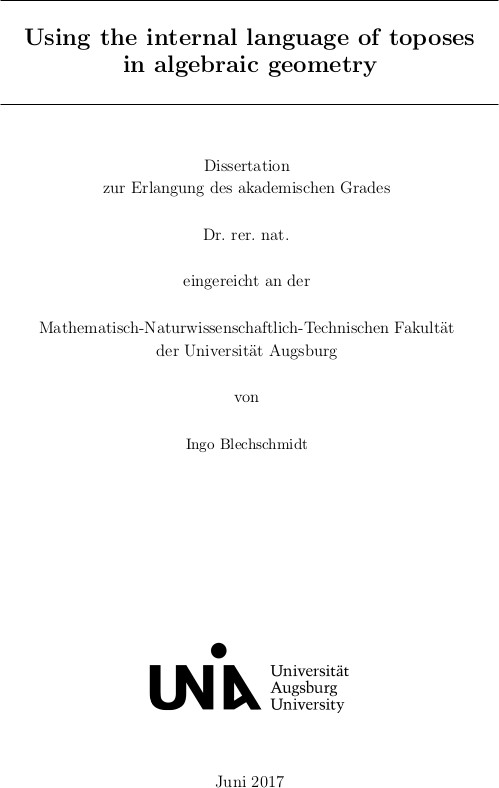
\includegraphics[height=0.8\textheight]{phd-cover}}}
  \par
\end{frame}

\begin{frame}{Applications in algebraic geometry}
  \vspace*{-1.5em}
  \begin{varblock}{0.9\textwidth}{}
    \justifying
    Understand \hil{notions of algebraic geometry} over a scheme~$X$ as
    \hil{notions of algebra} internal to~$\Sh(X)$.
  \end{varblock}

  \small\centering
  \scalebox{0.83}{\begin{tabular}{ll}
    \toprule
    externally & internally to $\Sh(X)$ \\
    \midrule
    sheaf of sets & set \\
    %sheaf of rings & ring \\
    sheaf of modules & module \\
    sheaf of finite type & finitely generated module \\
    % finite locally free sheaf & finite free module \\
    % coherent sheaf & coherent module \\
    tensor product of sheaves & tensor product of modules \\
    % sheaf of Kähler differentials & module of Kähler differentials \\
    sheaf of rational functions & total quotient ring of~$\O_X$ \\
    dimension of $X$ & Krull dimension of~$\O_X$ \\
    spectrum of a sheaf of~$\O_X$-algebras & ordinary spectrum [with a twist] \\
    higher direct images & sheaf cohomology \\
    \bottomrule
  \end{tabular}}

  \begin{columns}[c]
    \begin{column}{0.47\textwidth}
      \begin{exampleblock}{}
        \justifying
        Let $0 \to \F' \to \F \to \F'' \to 0$ be a short exact sequence
        of sheaves of~$\O_X$-modules. If~$\F'$ and~$\F''$ are of finite type,
        so is~$\F$.
      \end{exampleblock}
    \end{column}

    \begin{column}{0.1\textwidth}
      \vspace*{0.7em}
      \scalebox{3}{$\Leftarrow$}
    \end{column}

    \begin{column}{0.44\textwidth}
      \begin{exampleblock}{}
        \justifying
        Let~$0 \to M' \to M \to M'' \to 0$ be a short exact sequence of
        modules. If~$M'$ and~$M''$ are finitely generated, so is~$M$.
      \end{exampleblock}
    \end{column}
  \end{columns}
\end{frame}

\begin{frame}{Synthetic algebraic geometry}
  Usual approach to algebraic geometry: \hil{layer schemes above ordinary set theory}
  using either
  \begin{itemize}
    \item locally ringed spaces
    \small
    \begin{multline*}
      \text{set of prime ideals of~$\ZZ[X,Y,Z]/(X^n+Y^n-Z^n)$} + {} \\
      \text{Zariski topology} + \text{structure sheaf}
    \end{multline*}
    \normalsize
    \item or Grothendieck's functor-of-points account, where a scheme is a functor~$\mathrm{Ring} \to \mathrm{Set}$.
    \small\[ A \longmapsto \{ (x,y,z) \in A^3 \,|\, x^n+y^n-z^n=0 \} \]
  \end{itemize}
  \bigskip

  \hil{Synthetic approach:} model schemes \hil{directly as sets} in a certain
  nonclassical set theory, the internal universe of the \mbox{\hil{big Zariski
  topos}} of a base scheme.
  \small
  \[ \{ (x,y,z) \? (\affl)^3 \,|\, x^n+y^n-z^n=0 \} \]
\end{frame}

\fontsize{11pt}{13.2}

\begin{frame}{The big Zariski topos}
  Let~$S$ be a fixed base scheme.
  \begin{varblock}{0.9\textwidth}{Definition}
    The \hil{big Zariski topos} $\Zar(S)$ of a scheme~$S$ is equivalently
    \begin{enumerate}
      \item the topos of sheaves over~$(\Aff/S)_{\mathrm{lofp}}$,
      \item the classifying topos of local rings over~$S$ or
      \item the classifying~$\Sh(S)$-topos of local~$\O_S$-algebras which are
      local over~$\O_S$.
    \end{enumerate}
  \end{varblock}

  \begin{itemize}
    \item For an~$S$-scheme~$X$, its functor of points $\ull{X} =
    \Hom_S(\cdot,X)$ is an object of~$\Zar(S)$. It feels like \hil{the set of
    points} of~$X$.
    \item In particular, there is the ring object~$\affl$ with~$\affl(T) =
    \O_T(T)$.
    \item This ring object is a \hil{field}: nonzero implies
    invertible. \\{} [Kock 1976]
  \end{itemize}

  \jnote{1}{The objects of the category~$(\Aff/S)_{\mathrm{lofp}}$ are
  morphisms of the form~$\Spec(R) \to S$ which are locally of finite
  presentation. (Other choices of resolving set-theoretical issues of size are
  also possible.)

  A functor~$F : (\Aff/S)_{\mathrm{lofp}}^\op \to \Set$ is a sheaf
  for the Zariski topology if and only if the diagram
  \[ F(T) \to
    \prod_i F(U_i) \rightrightarrows
    \prod_{j,k} F(U_j \cap U_k) \]
  is a limit diagram for any open covering~$T = \bigcup_i U_i$ of any
  scheme~$T \in (\Aff/S)_{\mathrm{lofp}}$.

  In the case that~$S = \Spec(A)$ is affine, the big Zariski topos of~$S$ is also
  simply called ``big Zariski topos of~$A$''. It is a subtopos of the topos of
  functors $\mathrm{Alg}(A) \to \Set$ and classifies local~$A$-algebras.

  From the internal point of view of~$\Sh(S)$, the sheaf~$\O_S$ of rings is
  just an ordinary ring, and we can construct internally to~$\Sh(S)$ the big
  Zariski topos of~$\O_S$. Externally, this construction will yield a certain
  bounded topos over~$\Sh(S)$. However, as indicated on the slide, this topos
  will \emph{not} coincide with the true big Zariski topos of~$S$. To
  construct the true big Zariski topos, we have to build, internally
  to~$\Sh(S)$, the classifying topos of local \emph{and local-over-$\O_S$}
  $\O_S$-algebras.}
\end{frame}

\begin{frame}{Synthetic constructions}
  \small
  $\hil{$\boldsymbol{\mathbb{A}^n}$} = (\affl)^n = \affl \times \cdots \times \affl$

  $\begin{array}{@{}r@{}c@{}l@{}}
    \hil{$\boldsymbol{\mathbb{P}^n}$} &\phantom{}=\phantom{}& \{ (x_0,\ldots,x_n) : (\affl)^{n+1} \,|\, x_0 \neq 0 \vee
    \cdots \vee x_n \neq 0 \}/(\affl)^\times \\
    &\cong& \text{set of one-dimensional subspaces of~$(\affl)^{n+1}$} \\
    &&\qquad \text{(with~$\O(-1) = (\ell)_{\ell \? \mathbb{P}^n}$, $\O(1) =
    (\ell^\vee)_{\ell \? \mathbb{P}^n}$)}
  \end{array}$

  $\hil{$\boldsymbol{\Spec(R)}$} = \Hom_{\mathrm{Alg}(\affl)}(R, \affl) =
    \text{set of $\affl$-valued points of $R$}$

  $\hil{$\boldsymbol{TX}$} = X^\Delta$, where $\Delta = \{ \varepsilon \? \affl \,|\, \varepsilon^2 = 0 \}$

  A subset $U \subseteq X$ is \hil{qc-open} if and only if for any $x : X$
  there exist $f_1,\ldots,f_n \? \affl$ such that $x \in U \Longleftrightarrow
  \exists i\_ f_i \neq 0$.

  A \hil{synthetic affine scheme} is a set which is in bijection
  with~$\Spec(R)$ for some synthetically quasicoherent~$\affl$-algebra~$R$.

  A \hil{finitely presented synthetic scheme} is a set which can be covered by
  finitely many qc-open f.p. synthetic affine schemes~$U_i$ such that the
  intersections~$U_i \cap U_j$ can be covered by finitely many qc-open f.p.
  synthetic affine schemes.

  \jnote{1}{In the internal universe of the big Zariski topos of a base
  scheme~$S$, $S$-schemes can simply be modeled by sets (enjoying the special
  property that, in a certain precise sense, they are locally affine). This
  slide expresses some of the basic constructions of~$S$-schemes in that
  language.

  Particularly nice are the following items.
  \begin{itemize}\justifying
    \item Projective~$n$-space can be given by the any of the two quite naive
    expressions displayed on the slide.
    \item Let~$X$ be an~$S$-scheme. We often think about a sheaves
    of~$\O_X$-modules over~$X$ by their fibers; but for a rigorous
    treatment in the standard foundations, we have to take the full sheaf
    structure into account; the fibers do not determine a sheaf
    uniquely.

    From the internal point of view of~$\Zar(S)$, a sheaf of~$\O_X$-modules is
    indeed simply a family of~$\affl$-modules, one~$\affl$-module for each
    element of~$\ull{X}$. The slide illustrates how we can define the Serre
    twisting sheaves in this language.
  \end{itemize}}

  \jnote{2}{\begin{itemize}\justifying
    \item The spectrum of an~$\affl$-algebra can be given by the naive
    expression displayed on the slide. It looks like this expression can't be
    right, ignoring any non-maximal ideals; however, it is.
    \item The big Zariski topos of an~$S$-scheme~$X$ is, from the internal
    point of view of~$\Zar(S)$, simply the slice topos~$\Set/\ull{X}$. Hence to
    give an~$X$-scheme simply amounts to giving an~$\ull{X}$-indexed family of
    sets.
  \end{itemize}

  Synthetic algebraic geometry has been developed up to the point of étale
  geometric morphisms. Much remains to be done: For instance, as of yet there
  is only an account of Čech methods for computing cohomology, there is not yet
  a synthetic treatment of true cohomology. Derived categories and intersection
  theory are also missing.}
\end{frame}

\begin{frame}{Relations between the Zariski toposes}
  The big Zariski topos is a topos over the small Zariski topos:
  \[ \begin{array}{crcl}
    \pi : & \Zar(A) &\longrightarrow& \Spec(A) \\
    & \text{local~$A$-algebra~$(A \xrightarrow{\alpha} B)$} &\longmapsto& (A \to A[(\alpha^{-1}[B^\times])^{-1}])
  \end{array} \]
  This morphism is \hil{connected} ($\pi^{-1}$ is fully faithful) and
  \hil{local}, so there is a preinverse
  \[ \begin{array}{rcl}
    \Spec(A) &\longrightarrow& \Zar(A) \\
    \text{local localization~$(A \to B)$} &\longmapsto& (A \to B)
  \end{array} \]
  which is a subtopos inclusion inducing an idempotent monad~$\sharp$ and an
  idempotent comonad~$\flat$ on~$\Zar(S)$.

  \begin{itemize}
  \justifying
    \item Internally to~$\Zar(S)$, $\Spec(S)$ can be constructed as the
    \hil{largest subtopos} where~$\flat \affl \to \affl$ is bijective.
    \item Internally to~$\Spec(S)$, $\Zar(S)$ can be constructed as the
    \hil{classifying topos} of local~$\O_S$-algebras which are local over~$\O_S$.
    \item $\Zar(A)$ is the \hil{lax pullback}~$(\Set
    \Rightarrow_{\Set[\Ring]} \Set[\LocRing])$.
  \end{itemize}

  \jnote{1}{Let~$A$ be a ring. By definition, we obtain a geometric
  morphism~$\Set \to \Set[\Ring]$ into the classifying topos of rings.
  There is also a geometric morphism~$\Set[\LocRing] \to \Set[\Ring]$, obtained
  by realizing that any local ring is in particular a ring. These morphisms fit
  together in a lax pullback square as follows:
  \[ \xymatrix{
    \Zar(A) \ar[r] \ar[d] & \Set[\LocRing] \ar[d] \\
    \Set \ar[r] \ar@{}[ur]^(.3){}="a"^(.7){}="b" \ar@{=>} "a";"b" & \Set[\Ring]
  } \]
  This observation is joint with Peter Arndt and Matthias Hutzler.

  Incidentally, the pseudo pullback of the morphism~$\Set[\LocRing] \to
  \Set[\Ring]$ along~$\Set \to \Set[\Ring]$ is not very interesting: It's the
  largest subtopos of~$\Set$ where~$A$ is a local ring. Assuming the law of
  excluded middle, this subtopos is either the trivial topos (if~$A$ is not
  local) or~$\Set$ (if~$A$ is local).

  There is also a way of realizing the little Zariski topos of~$A$ as a pseudo
  pullback, exploiting that the (localic) spectrum construction is geometric.
  See Section~12.6 of
  \fixedhref{https://rawgit.com/iblech/internal-methods/master/notes.pdf}{these
  notes} for details.
  }
\end{frame}


\section{The mystery of nongeometric sequents}

\begin{frame}{Properties of the affine line}
  \begin{itemize}
%   \item $\affl$ is a local ring:
%   \[ 1 \neq 0 \qquad\qquad \text{$x + y$ \inv} \Longrightarrow \text{$x$ \inv} \vee
%   \text{$y$ \inv} \]
    \item $\affl$ is a field:
    \begin{align*}
      \neg(x = 0) &\Longleftrightarrow \text{$x$ invertible \quad [Kock 1976]} \\
      \neg(\text{$x$ invertible}) &\Longleftrightarrow \text{$x$ nilpotent}
    \end{align*}
    \item $\affl$ satisfies the axiom of microaffinity: Any map $f : \Delta \to
    \affl$ is of the form~$f(\varepsilon) = a + b \varepsilon$ for unique
    values~$a,b \? \affl$, where~$\Delta = \{ \varepsilon \? \affl \,|\,
    \varepsilon^2 = 0 \}$.
    \bigskip
    \item Any map $\affl \to \affl$ is a polynomial function.
    \bigskip
    \item $\affl$ is anonymously algebraically closed: Any monic polynomial
    does \emph{not not} have a zero.
  \end{itemize}

  \jnote{1}{The axiom of microaffinity is a special instance of the
  \emph{Kock--Lawvere axiom} known from synthetic differential geometry. We'll
  see on the next slide that~$\affl$ validates an unusually strong form of the
  Kock--Lawvere axiom, not at all satisfied in the usual well-adapted models of
  synthetic differential geometry.

  The fact that, internally to~$\Zar(S)$, any map~$\affl \to \affl$ is a
  polynomial can be seen as a formal version of the general motto that in
  algebraic geometry, ``morphisms are polynomials''.}
\end{frame}

\begin{frame}{Synthetic quasicoherence}
  Recall~$\Spec(R) = \Hom_{\mathrm{Alg}(\affl)}(R, \affl)$ and consider the statement
  \[ \text{``the canonical map~$
    \begin{array}[t]{rcl}
      R &\longrightarrow& (\affl)^{\Spec(R)} \\
      f &\longmapsto& (\alpha \mapsto \alpha(f))
    \end{array}
  $ is bijective''}.
  \]
  \vspace*{-1em}

  \begin{itemize}
    \item True for~$R = \affl[X]/(X^2)$ (microaffinity).
    \item True for~$R = \affl[X]$ (every function is a polynomial).
    \item True for \hil{any} finitely presented~$\affl$-algebra~$R$.
  \end{itemize}

  Any known property of~$\affl$ follows from this \\
  \hil{synthetic quasicoherence}.

  \centering
  \begin{varblock}{0.6344\textwidth}{}
    \centering
    \hil{the mystery of nongeometric sequents}
    \par
  \end{varblock}

  \jnote{1}{Let~$R$ be an~$\affl$-algebra. An element~$f \in R$ induces
  an~$\affl$-valued function on~$\Spec(R)$; functions of this form can
  reasonably be called ``algebraic''. In a synthetic context, there should be
  no other~$\affl$-valued functions on~$\Spec(R)$ as these algebraic ones, and
  different algebraic expressions should yield different functions. This is
  precisely what the bijectivity of the displayed map expresses (in a positive
  way).

  In synthetic differential geometry, the closest cousin of synthetic algebraic
  geometry, the analogue of the displayed map is only bijective for Weil
  algebras such as~$\affl[X]/(X^2)$ or $\affl[X,Y]/(X^2,XY)$, not for arbitrary
  finitely presented~$\affl$-algebras. This is a major difference to synthetic
  differential geometry.}

  \jnote{2}{The notion of synthetic quasicoherence is interesting for a number
  of reasons:\vspace*{-1.2em}
  \begin{itemize}\justifying
    \item All currently known properties of~$\affl$, such as all the properties
    listed on the previous slide, follow from the statement that~$\affl$ is
    synthetically quasicoherent.

    For instance, here is how we can verify the field property. Let~$x \?
    \affl$ such that~$x \neq 0$. Set~$R = \affl/(x)$. Then~$\Spec(R) =
    \emptyset$. Thus~$(\affl)^{\Spec(R)}$ is a singleton. Hence~$R = 0$.
    Therefore~$x$ is invertible.
    \item Given an~$\affl$-module~$E$, we can formulate the following variant
    of the axiom of synthetic quasicoherence: ``For any finitely
    presented~$\affl$-algebra~$R$, the canonical map~$R \otimes_\affl E \to
    E^{\Spec(R)}$ is bijective.'' This axiom is satisfied if and only if~$E$ is
    induced by a quasicoherent sheaf of~$\O_S$-modules.
    \item The notion of synthetic quasicoherence is central to synthetic
    algebraic geometry. The notions of synthetic open immersions, closed
    immersion, schemes and several others all refer to synthetic
    quasicoherence.
  \end{itemize}}

  \jnote{3}{An analogue of synthetic quasicoherence holds in the classifying
  topos of rings, demonstrating that even presheaf toposes can validate
  interesting nontrivial nongeometric sequents.

  We believe that an analogue of synthetic quasicoherence holds for the generic
  model of any geometric theory. This is work in progress. If true, this would
  yield a major source of nongeometric sequents in classifying toposes. Because
  of the many applications on nongeometric sequents, it's very desirable to
  possess such a source.

  The mystery of nongeometric sequents is this: On the one hand, they are very
  useful to have because of surprising applications; on the other hand, they
  are as of yet quite elusive.}
\end{frame}

\fontsize{10pt}{12}
{\usebackgroundtemplate{\begin{minipage}{\paperwidth}\vspace*{4.95cm}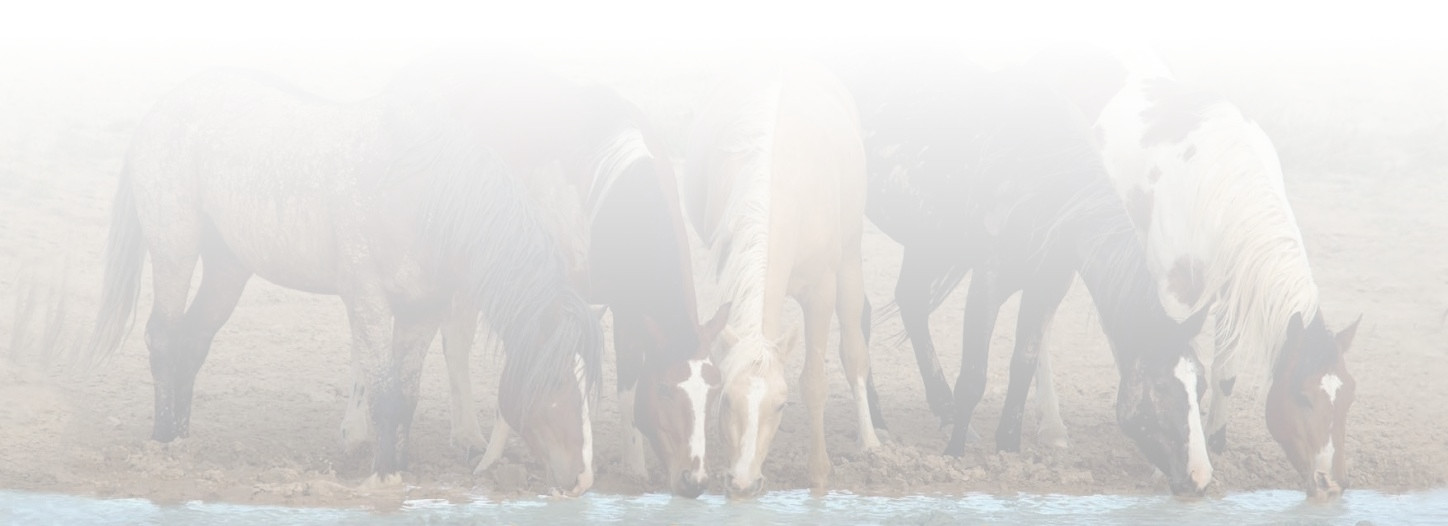
\includegraphics[width=\paperwidth]{topos-horses-lighter}\end{minipage}}
\begin{frame}{\!\!\!\mbox{Classifying toposes in algebraic geometry}}
  \footnotesize
  \centering
  \begin{tabular}{ll}
    \toprule
    (big) topos & classified theory \\\midrule
    Zariski & local rings [Hakim 1972] \\[0.6em]
    étale & separably closed local rings [Hakim 1972, Wraith 1979] \\[0.6em]
    \usebeamercolor[fg]{item}{fppf} & \usebeamercolor[fg]{item}{fppf-local rings} \\
    & \textcolor{red!90}{(conjecturally: algebraically closed local rings)} \\[0.6em]
    \textcolor{red!80}{ph} & \textcolor{red!80}{?? (conjecturally: algebraically closed valuation rings} \\
    & \qquad \textcolor{red!80}{validating the projective Nullstellensatz)} \\[0.6em]
    \usebeamercolor[fg]{item}{surjective} & \usebeamercolor[fg]{item}{algebraically closed geometric fields} \\[0.6em]
    \textcolor{red!80}{$\neg\neg$} & \textcolor{red!80}{?? (conjecturally: algebraically closed geometric} \\
    & \qquad \textcolor{red!80}{fields which are integral over the base)} \\[0.6em]
    \usebeamercolor[fg]{item}{infinitesimal} & \usebeamercolor[fg]{item}{local algebras together with a nilpotent ideal [Hutzler 2018]} \\[0.6em]
    \textcolor{red!100}{crystalline} & \textcolor{red!100}{??} \\
    \bottomrule
  \end{tabular}

  \jnote{1}{Toposes, and also more specifically classifying toposes, originated
  in algebraic geometry. It is therefore deeply embarrassing that as of now,
  still very little is known about the theories classified by the major toposes
  in active use by algebraic geometers.
  \begin{center}
    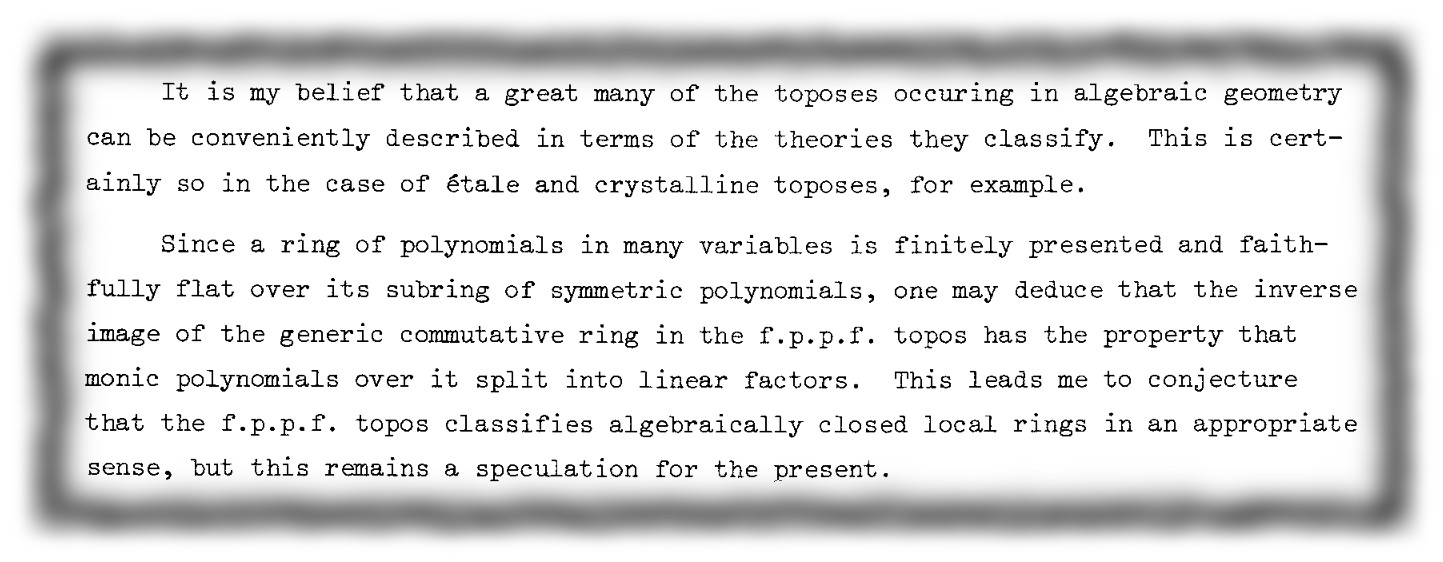
\includegraphics[width=0.99\textwidth]{wraith-generic-galois-theory} \\
    \footnotesize
    Gavin Wraith. Generic Galois theory of local rings. 1979. \\
    (A cult classic and must-read for anyone interested in \\
    the intersection of topos theory and algebraic geometry.)
  \end{center}}

  \jnote{2}{For almost forty years, only the big Zariski topos and its étale
  subtopos were understood in that way.
  \fixedhref{https://rawgit.com/iblech/internal-methods/master/notes.pdf}{These~2017
  notes} answer the question for the fppf topology and the surjective topology
  (in Section~21) and state conjectures for the ph topology and the
  double negation topology. However, while good to have, the answer for the
  fppf topology remains unsatisfactory, since Wraith's conjecture that the fppf
  topos classifies the simpler theory of algebraically closed local rings has
  neither been confirmed nor refuted.

  A couple of weeks ago, Matthias Hutzler managed to determine the theory
  classified by the big infinitesimal topos of a ring~$A$: It classifies
  pairs~$(B,\aaa)$ consisting of a local~$A$-algebra~$B$ and a nilpotent
  ideal~$\aaa \subseteq B$. Details will be in his forthcoming Master's thesis.
  He is currently working on answering the question for the closely related big
  crystalline topos.

  It will be exciting to learn what the crystalline topos and the many other
  toposes in algebraic geometry classify; how algebraic geometry can profit
  from these discoveries; and which new flavors of synthetic algebraic geometry
  they unlock.}
\end{frame}}
\backupend

\end{document}
